\appendix
\section{Supplementary experimental details}
\label{app:experimental_details}

\subsection{Implementation settings}
\label{app:implementation_settings}
\begin{table}[!htbp]
\centering
\fontsize{9pt}{11pt}\selectfont
\caption{Parameter settings for POI visit forecasting and attribution.}
\label{tab:parameter_settings}
\setlength{\tabcolsep}{5pt}
\renewcommand{\arraystretch}{1.12}
\begin{tabularx}{\linewidth}{@{}
>{\raggedright\arraybackslash}p{0.34\linewidth}
>{\raggedright\arraybackslash}X@{}}
\toprule
Parameter & Value \\
\midrule
Training / validation / test
& Oct.~1--Nov.~19 / Nov.~20--Dec.~3 /
Dec.~4--31, 2020 \\

Later-month evaluation & Jan.~1--31, 2021 \\

\addlinespace[2pt]
KNN neighbors \(k\)
& 10 \\

Controlled semantic and random graphs & \(k\in\{5,10,20\}\); matched degree per POI \\

Adaptive MTGNN graph & 20 selected neighbors per POI \\

RBF bandwidth \(\sigma\) and cutoff
& 1 km and 2 km \\

Visit-correlation threshold \(\eta_c\)
& 0.30 \\

\addlinespace[2pt]
Ridge penalty
& AR-ridge: \(\{1,10,100,1000\}\); validation selected \\

Hidden dimensions
& GraphGRU: 32;
GNN-static: 32;
LSTM: 32 \\

MTGNN architecture
& 3 temporal layers; graph depth 2; convolution/residual channels 32, skip channels 64, output channels 128 \\

MTGNN dropout / neural gradient clipping
& 0.1 / maximum gradient norm 5 \\

Neural learning-rate candidates
& \(\{3\times10^{-4},10^{-3},3\times10^{-3}\}\) \\

Batch size / optimizer
& 4 / Adam, weight decay \(10^{-4}\) \\

Training seeds & 42, 43, 44, 45, 46 \\

\addlinespace[2pt]
Recent-density window \(L_{\mathrm{rec}}\)
& 14 days \\

Density exclusion quantiles
& \(\{0.10,0.25,0.50,0.75\}\) \\

Low-history thresholds
& \(\eta_z=0.70\), \(\alpha=0.25\) \\

Graph-lift threshold \(\eta_G\)
& 0.1 \\

False-activation threshold \(\eta_{\mathrm{FAR}}\)
& 0.5 \\

Static-feature dimensions \(D_s\)
& 52 \\
\bottomrule
\end{tabularx}
\end{table}


\subsection{Checkpoint replay and numerical verification}
\label{app:checkpoint_replay}
January evaluation reconstructs each fitted checkpoint and first replays its archived validation and December forecasts.
The pointwise check uses relative and absolute tolerances of $2\times10^{-4}$.
For 19 MTGNN checkpoints, repeated graph operations exposed FP32 summation variation; deterministic graph evaluation with FP64 accumulation produced identical December and January predictions in two independent processes.
For these checkpoints, the supplementary numerical check bounds the change in cohort and per-lead MAE by $0.00005$ visits and the change in FAR, recall, and precision by $0.01$ percentage points across the five activation thresholds.
The measured maxima were $0.00000144$ visits and $0.00750$ percentage points, respectively.
The archive retains the original pointwise-check results, operator checks, and both independent prediction runs.
Validation calibration uses the archived predictions unchanged, and January retains the fitted parameters and selection choices.

\subsection{Descriptive attribution profiles}
\label{app:descriptive_attribution}
Figure~\ref{fig:attribution_fingerprint} summarizes the five-seed Gradient \(\times\) Input consensus at \(T=14\), \(H=7\).
The history-driven regime contains 3,495 POIs, followed by 2,094 identity-driven, 1,895 parent-driven, 1,219 others-driven, and 1,150 location-driven POIs; 31 POIs have zero total attribution in every fit and remain unassigned.
These labels identify the largest standardized share, not necessarily the largest original share.
All POIs in the parent-driven regime use the learned missing-parent category.
Table~\ref{tab:attri_regime} reports forecasting error within each regime, while Table~\ref{tab:category_regime_mae} describes their distribution across POI categories.
Under this attribution rule, restaurants and cafes are predominantly identity-driven, whereas history-driven assignments are more common among clinics and repair services.
Figure~\ref{fig:attribution_regime_map} maps these descriptive assignments.

\begin{figure}[!htbp]
\centering
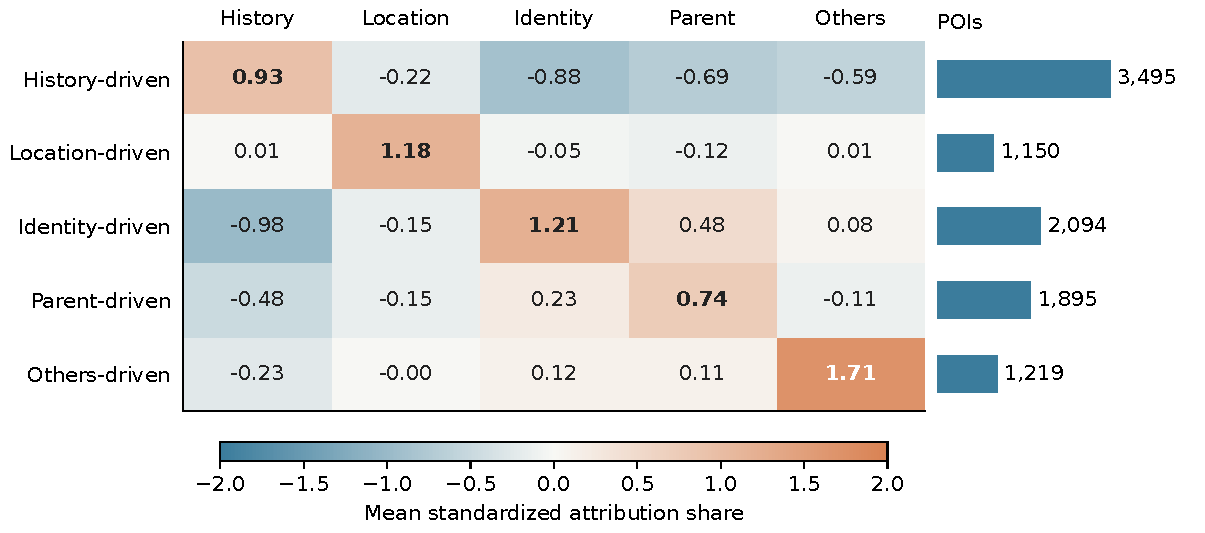
\includegraphics[scale=0.70]{art/attribution_fingerprint.pdf}
\caption{Mean standardized attribution shares and POI counts for the December five-seed consensus at \(T=14\), \(H=7\). Bold values identify the source defining each regime.}
\label{fig:attribution_fingerprint}
\end{figure}

\begin{table}[!htbp]
\centering
\begingroup
\singlespacing
\fontsize{9pt}{10.5pt}\selectfont
\setlength{\tabcolsep}{4pt}
\renewcommand{\arraystretch}{1.08}
\caption{December attribution regimes obtained from the five-seed consensus at $T=14$, $H=7$. Recorded parent counts POIs with an observed containing-place identifier. MAE averages the absolute errors of each fitted model over the same POIs and all test events.}
\label{tab:attri_regime}
\begin{adjustbox}{max width=\linewidth}
\begin{tabular}{lrrr}
\toprule
Regime & POIs & Recorded parent & MAE \\
\midrule
History-driven & 3,495 & 259 & 1.460 \\
Location-driven & 1,150 & 46 & 1.527 \\
Identity-driven & 2,094 & 132 & 1.218 \\
Parent-driven & 1,895 & 0 & 0.964 \\
Others-driven & 1,219 & 144 & 1.329 \\
\bottomrule
\end{tabular}
\end{adjustbox}
\endgroup
\end{table}

\begin{table}[!htbp]
\centering
\begingroup
\singlespacing
\fontsize{9pt}{10.5pt}\selectfont
\setlength{\tabcolsep}{4pt}
\renewcommand{\arraystretch}{1.08}
\caption{December regime shares (\%) within broad POI categories. H, L, I, P, and O denote history-driven, location-driven, identity-driven, parent-driven, and others-driven, respectively. Shares use assigned POIs; MAE uses all POIs in the category.}
\label{tab:category_regime_mae}
\begin{adjustbox}{max width=\linewidth}
\begin{tabular}{lrrrrrrr}
\toprule
POI category & POIs & H & L & I & P & O & MAE \\
\midrule
Schools, campuses, and education-related POIs & 294 & 45.1 & 22.2 & 1.7 & 19.5 & 11.6 & 1.237 \\
Repair, towing, and irregular services & 283 & 58.5 & 13.5 & 4.3 & 14.2 & 9.6 & 0.807 \\
Restaurants and cafes & 2,604 & 14.4 & 6.0 & 59.8 & 7.2 & 12.5 & 1.372 \\
Shopping centers and office-building POIs & 2,879 & 39.0 & 14.6 & 6.7 & 26.6 & 13.0 & 1.298 \\
Clinics and medical services & 1,090 & 59.4 & 12.1 & 4.4 & 15.5 & 8.7 & 1.312 \\
Pharmacies and health-related retail & 240 & 27.5 & 15.8 & 8.8 & 26.7 & 21.2 & 1.399 \\
Small local businesses & 1,688 & 45.5 & 13.7 & 4.5 & 27.6 & 8.7 & 1.302 \\
Bars and nightlife POIs & 383 & 14.9 & 3.9 & 37.7 & 22.5 & 20.9 & 1.020 \\
Grocery and daily retail & 423 & 41.6 & 13.4 & 9.3 & 15.1 & 20.6 & 1.425 \\
\bottomrule
\end{tabular}
\end{adjustbox}
\endgroup
\end{table}


\begin{figure}[!htbp]
\centering
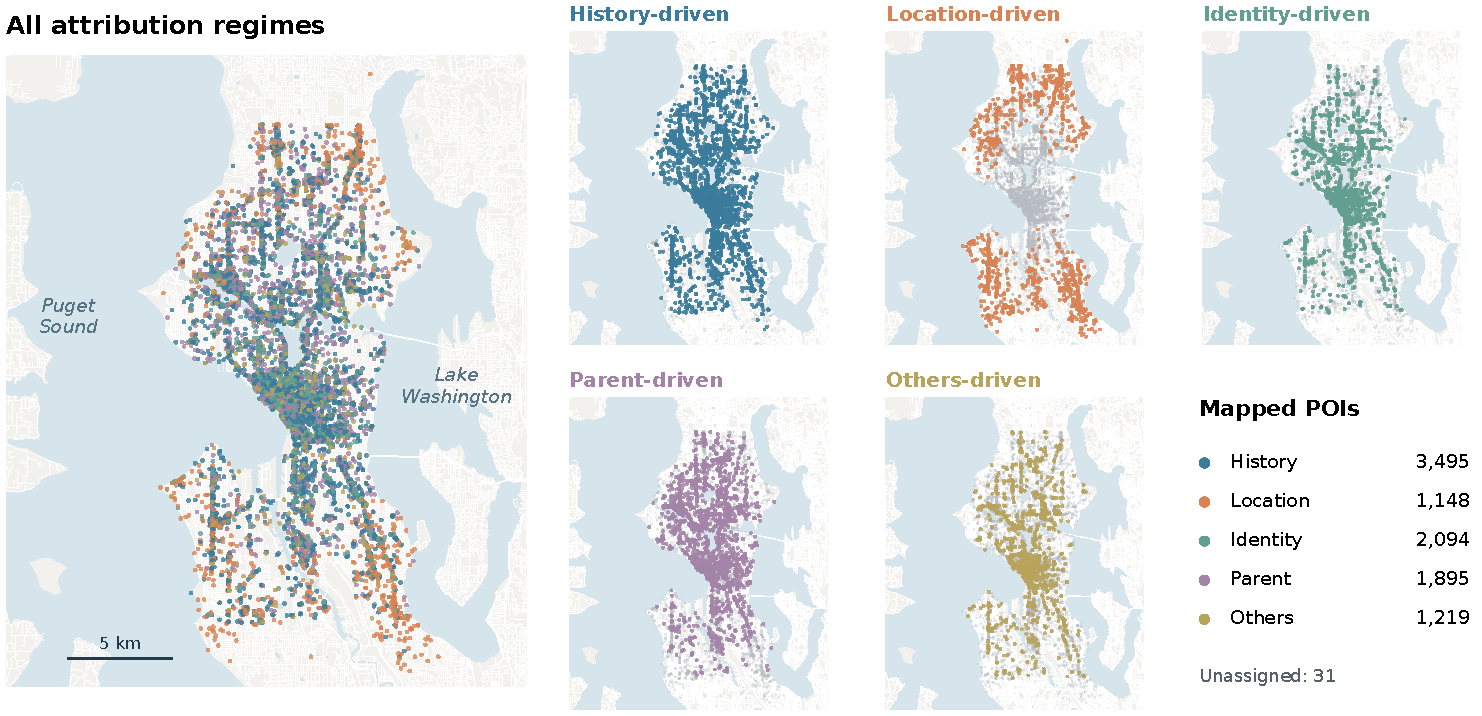
\includegraphics[scale=0.62]{art/attribution_cluster_map.pdf}
\caption{Spatial distribution of the December five-seed attribution consensus. The overview shows all regimes; each small panel highlights one regime against the other POIs. Gray also marks unassigned POIs. Counts refer to the mapped extent. Roads and water are from the 2020 U.S. Census Bureau TIGER/Line files.}
\label{fig:attribution_regime_map}
\end{figure}

